\documentclass[12pt, a4paper, titlepage]{article}
\usepackage{graphicx, amsmath, amsfonts, listings, amssymb, mathrsfs, color, fancyhdr, geometry, hyperref}
\usepackage[english]{babel}
\usepackage[utf8x]{inputenc}
\usepackage{wrapfig}
\graphicspath{ {images/} }
\usepackage[toc,page]{appendix}

\geometry{
a4paper,bindingoffset=0.2in,
            left=1in,right=1in,top=1in,bottom=1in,
            footskip=.25in
 }
\definecolor{mygreen}{RGB}{28,172,0}
\definecolor{mylilas}{RGB}{170,55,241}
\pagestyle{fancy}
\fancyhf{}
\rhead{Ashish T., Nischal L.S., Sagar D.}
\lhead{Election Portal}
\fancyfoot[C]{Page \thepage}
\renewcommand{\headrulewidth}{2pt}

\begin{document}


\begin{titlepage}
\newcommand{\HRule}{\rule{\linewidth}{0.5mm}}
\center
\begin{center}
	
\includegraphics[scale=0.4]{ncit}
\end{center}
\vspace{0.75cm}
 \textsc{\Large \textbf{Nepal College of Information Technology}}\\
{\large \textbf{Web Design Competition} \par}
\vfill
\HRule \\[0.4cm]

\includegraphics[scale=0.4]{logo.png}\\[1cm] 
{ \huge \bfseries Election Portal}\\
\textsc{\large Discover everything election!}
\HRule \\[1.5cm]
\vfill
{\large Team members}\\
{\Large \textbf{Ashish Tiwari} \par}
{\Large \textbf{Nischal Lal Shrestha} \par}
{\Large \textbf{Sagar Devkota} \par}
\vfill
{\large \today}\\[1cm] 
\end{titlepage}

\pagenumbering{roman}

\section*{Abstract}
\addcontentsline{toc}{section}{Abstract}
\thispagestyle{empty}
The purpose of Election Portal is to digitize election and election-related activities in Nepal. Election Portal, therefore, offers a web application which stores candidate information, election constituency details, latest election results, and various other information directly related to election and enables the clients to fetch those data efficiently. The problem statement relies on understanding proper way to store all those dataset in the database, solving the complexity involved within and finding an appropriate interface to provide all these dataset to the visitors. Election Portal also provides opportunity to individual volunteers who are authorized to update election result dataset of a particular constituency in real-time. Each web page of the Election Portal is equipped with either a search form or a filter form to enhance user's ability to get information very quickly.
\\
% Keywords command
\providecommand{\keywords}[1]
{
  \small    
  \textbf{\textit{Keywords---}} #1
}

\hspace{10pt}
\keywords{Datasets, Django, Election, Portal, Web Application}

\newpage

\tableofcontents
\newpage

\pagenumbering{arabic}

\section{Introduction}
Elections are hold on virtually every part of the world today to select an individual by a population to hold public office in a modern democracy. This system has been around from 17th century and it may be observed to fill offices in the legislature, executive and judiciary, and for regional and local government. In Nepal, elections are observed on three levels: Federal parliament, state assemblies and for the local government. \\ \\
Election Portal is a web application for individual visitors, journalists, students to get election results and other election-related activities at a single place. Election Portal will provide opportunity to individual volunteers to update the election datasets, election result in a real time.

\section{Problem Statement}
The problem statement for Election Portal is based on understanding and developing a effective way to store all the datasets of election-related activities in a profound way, solving all the complexity involved with the datasets. It also relies on building a interface to filter and search the election datasets through the database in a effective manner.

\section{SCOPE AND IMPORTANCE}

\newpage
\section{UML Design}
\subsection{Use Case Diagram}
\begin{figure}[ht]
	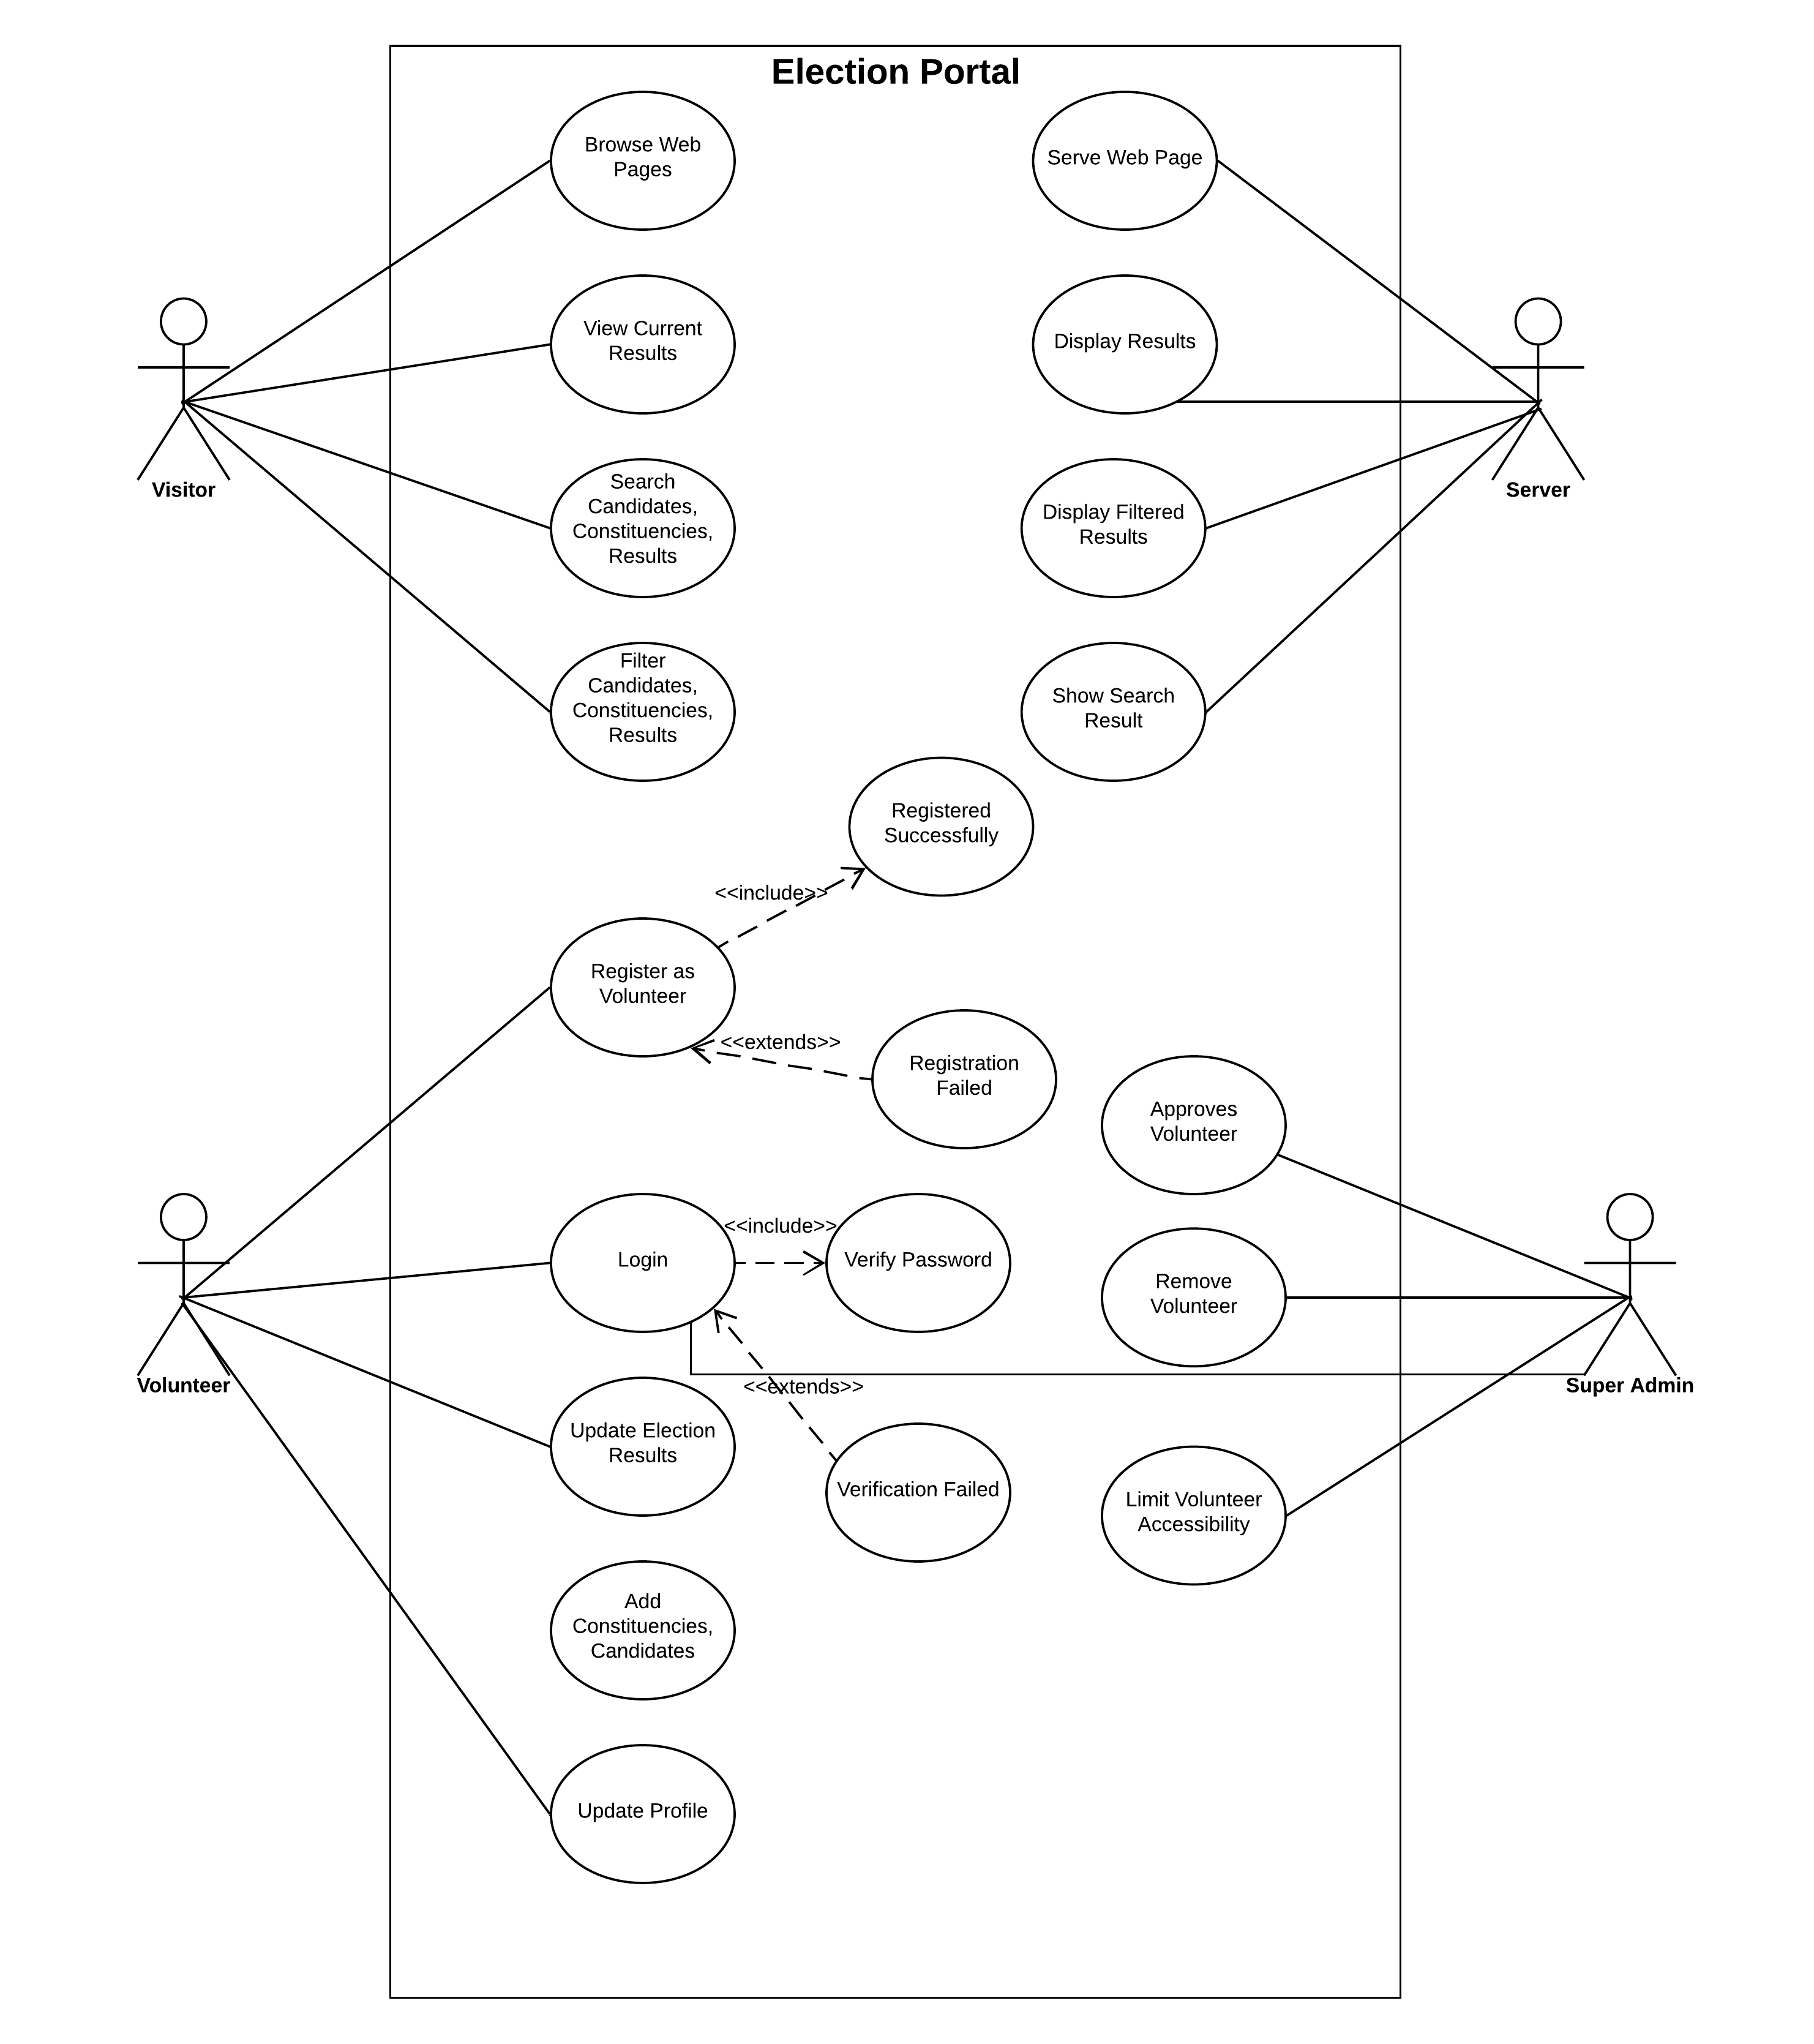
\includegraphics[scale=0.6]{election_portal_use_case_diagram.png}
	\caption{Use Case Diagram of Election Portal}
\end{figure}
The use case diagram of Election Portal contains the scope of the system and it lists all the functionalities offered by the system. We have identified the following actors:

\subsubsection{Visitor}
Visitor represents as the primary actor for this system. Vistors can browse web pages, view current results, search and filter candidates, constituencies, results.

\subsubsection{Volunteer} 
Volunteer act to update election results, add new datasets in the system. Volunteer needs to register first and then login to make changes in the system.

\subsubsection{Super Admin}
Super Admin regulates the database. Super Admin approves new volunteer, remove volunteer and limit their access to the database.

\subsubsection{Server} 
A Server act to store the volunteers authentications information. Server acts to provides the web pages and datasets from database to users on their requests throuh a web browser. \\ \\
Based on the above use case diagram, the following group of activities have been identified.
\begin{enumerate}
\item Visitors enters the web portal and browse various web pages.
\item Visitors can either search or filter the datasets through form.
\item Volunteer can Create, Read, Update and Delete datasets from the database.
\item Super Admin can approve new volunteer, limit access to volunteer and delete existing volunteer.
\end{enumerate}

\newpage	
\subsection{UML Class Diagram}
\begin{center}
\begin{figure}[ht]
	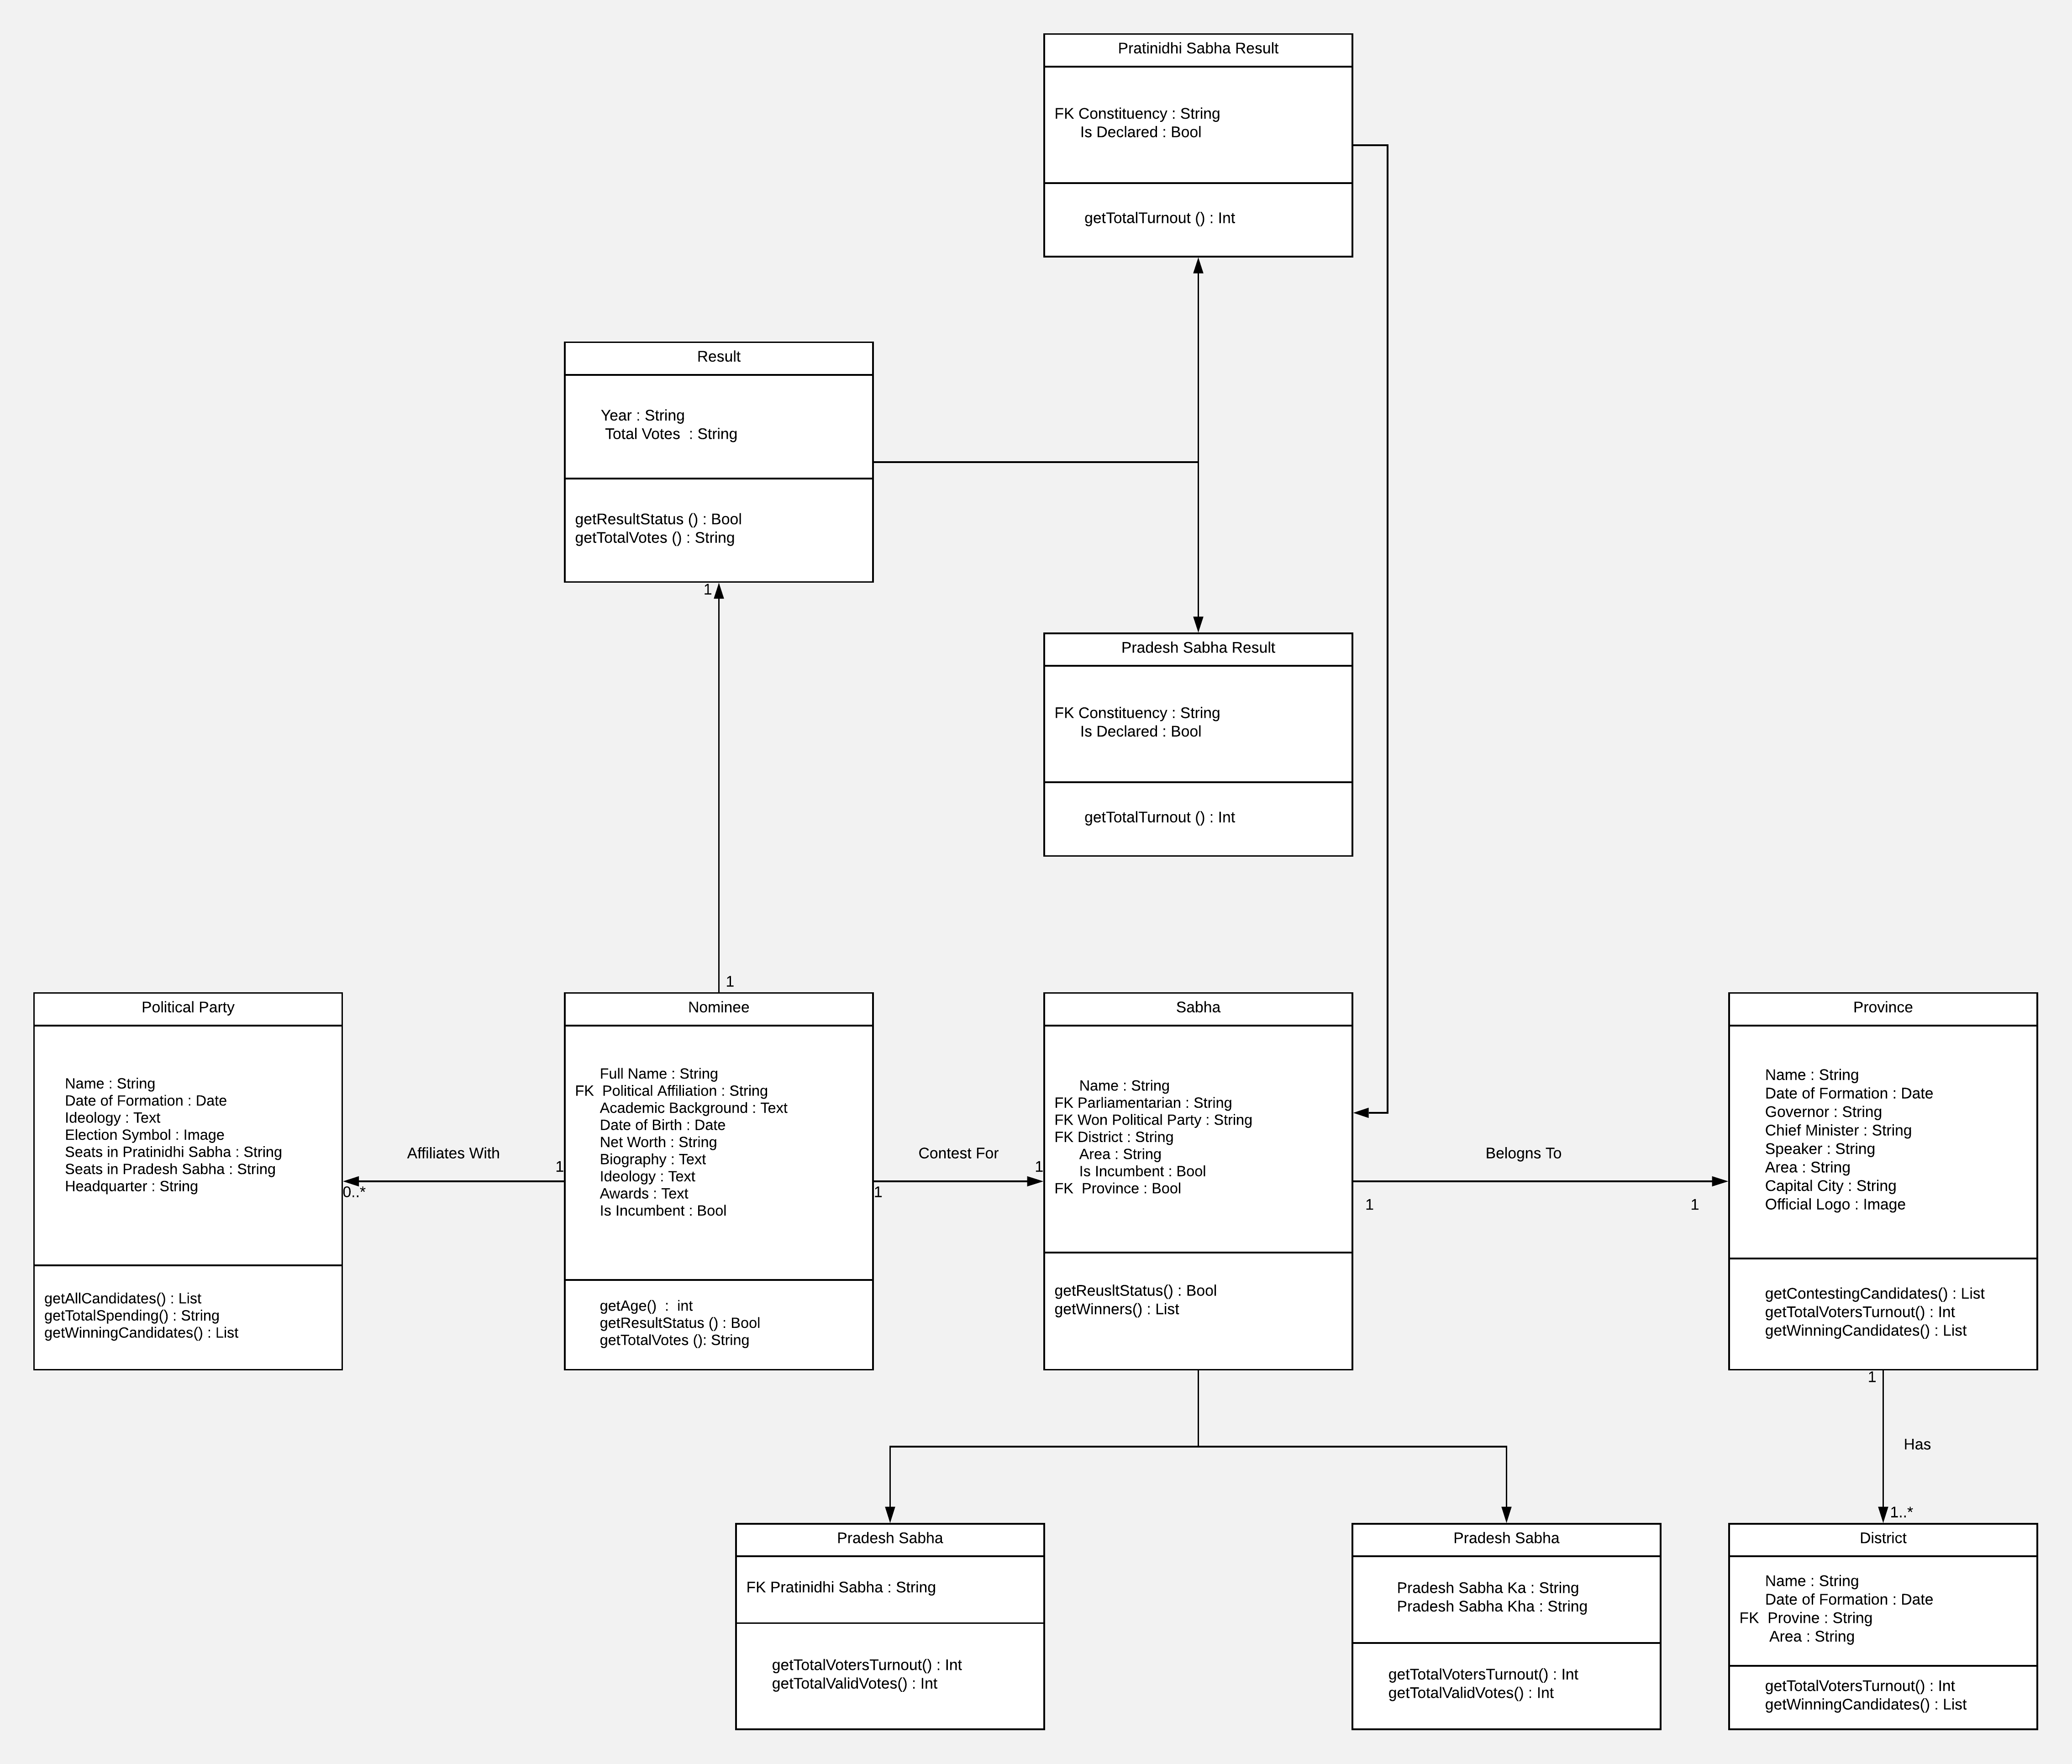
\includegraphics[scale=0.45]{Class_Diagram_for_Election_Portal_1.png}
	\caption{Class Diagram of Nominee}
\end{figure}
\end{center}

\begin{center}
\begin{figure}
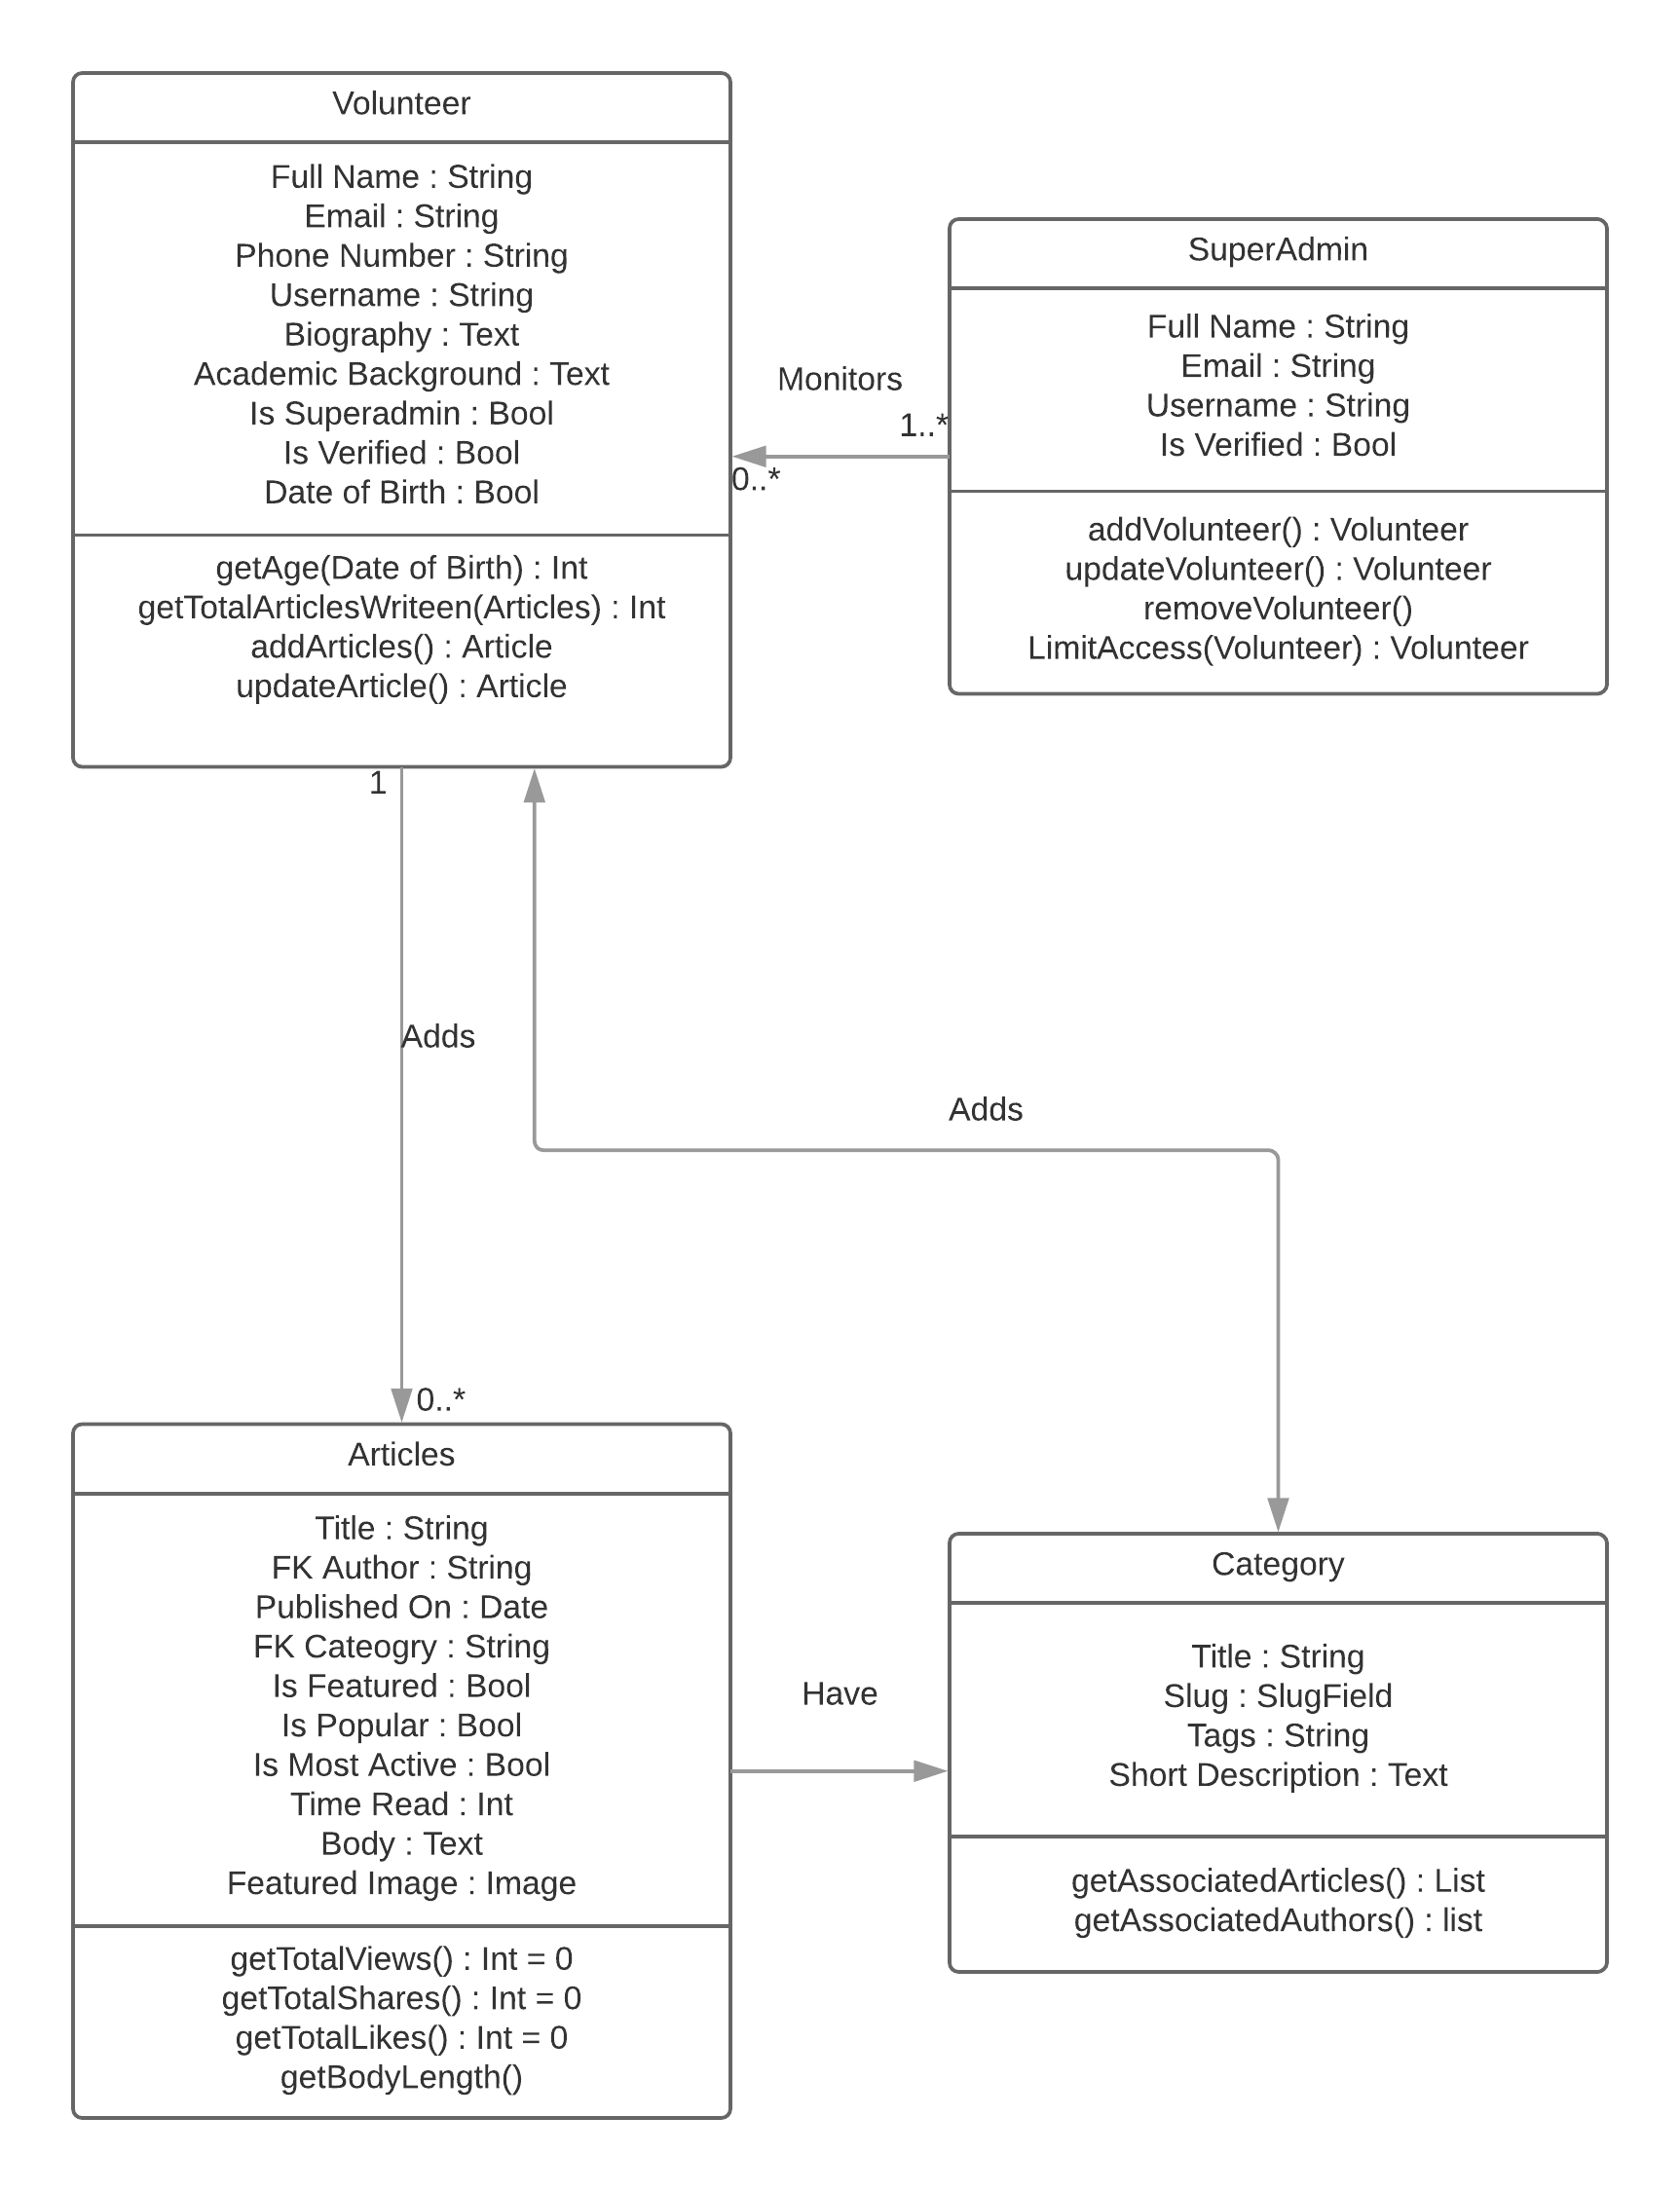
\includegraphics[scale=0.5]{Class_Diagram_for_Election_Portal_2.png}
	\caption{Class Diagram for Article and Volunteer}
\end{figure}
\end{center}

\section{TASK AND TIME SCHEDULE}
\subsection{GANTT Chart }
\newpage

\section{Framework of the Development}
\subsection{Logical Architecture Diagram}
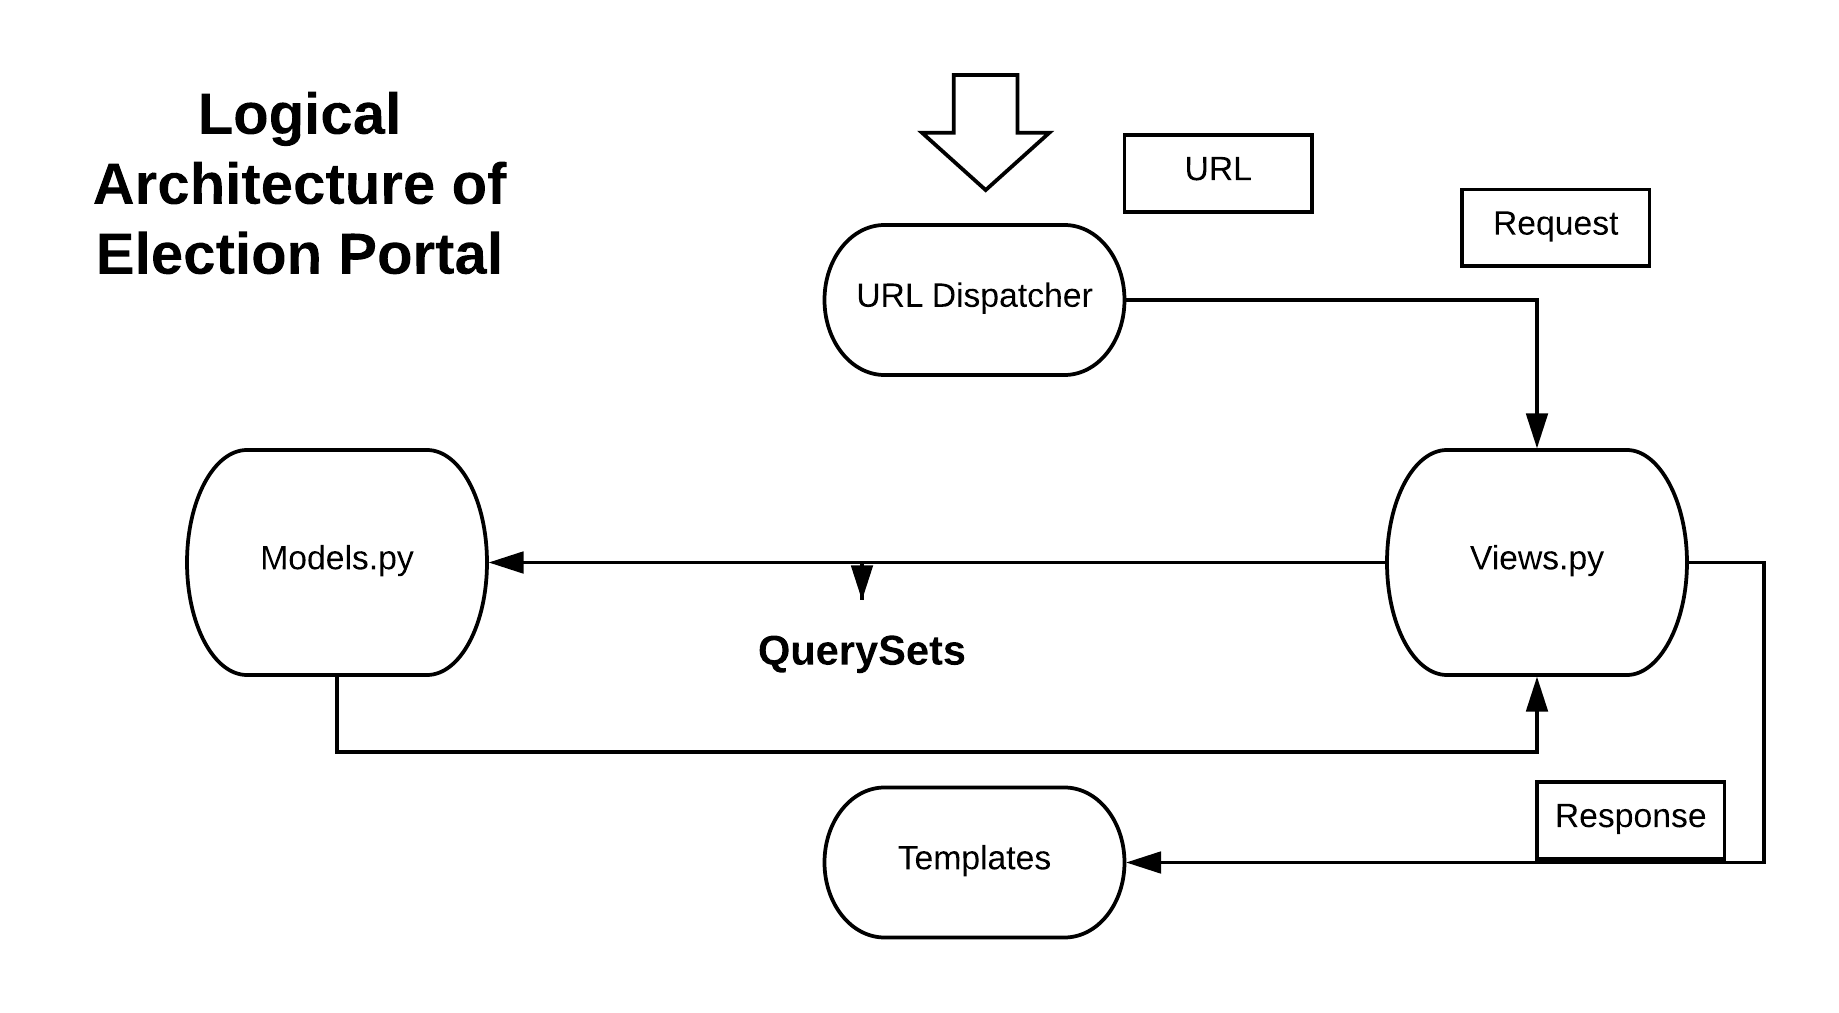
\includegraphics[scale=0.8]{Logical_Architecture.png}\\
There are three layers between User Interface and Database. Those are:
\begin{enumerate}
\item Data Access Layer(models.py)\\
This layers defines everything about the data: how to access data, how we can validate data, what type of behaviors our data will show, and what type of relationship exists between different data.
\item Presentation Layer(Templates)\\
Presentation layer will define how something should be displayed on a Web Page. Presentation layer takes information from the database and display it to the user in a Human-Understandable-Format. Presentation layer is completely free of any king of logic.
\item Business Logic Layer(views.py)\\
Business Logic Layer is a bridge between models and templates. It provides appropriate way to supply specific templates requested by the data access layer.
\end{enumerate}
\newpage

\section{Tools and Technology Used}

\begin{enumerate}
\item Django\\
We had used Django 2.0.7 to handle backend of Election Portal.
Django is a high-level Python Web framework that encourages rapid development and clean, pragmatic design. Built by experienced developers, it takes care of much of the hassle of Web development, so you can focus on writing your app without needing to reinvent the wheel. It’s free and open source

\item 
U.S. Web Design System\\
A design system for the federal government. The design standards by US Web Design System are backed by user research.

\item SQLite\\
SQLite is already installed in Django. So we did not install it from outside. SQLite is a self-contained, high-reliability, embedded, full-featured, public-domain, SQL database engine. SQLite is the most used database engine in the world.

\item JQuery\\
We had used JQuery 3.3.1 in out project. JQuery is a fast and concise JavaScript Library created by John Resig in 2006 with a nice motto: Write less, do more. jQuery simplifies HTML document traversing, event handling, animating, and Ajax interactions for rapid web development.

\item HTML and CSS\\
HTML, HyperText Markup Language, gives content structure and meaning by defining that content as, for example, headings, paragraphs, or images. CSS, or Cascading Style Sheets, is a presentation language created to style the appearance of content—using, for example, fonts or colors.
\end{enumerate}
\newpage

    
\section{Graphical User Interface of the System}
Election Portal has a GUI so that visitors can easily browse the portal with the least effort. Every page has a header and footer. The header consists of the Navigation menu so that visitors can navigate throughout the webpage without being lost.
\subsection{Homepage}
\begin{center}
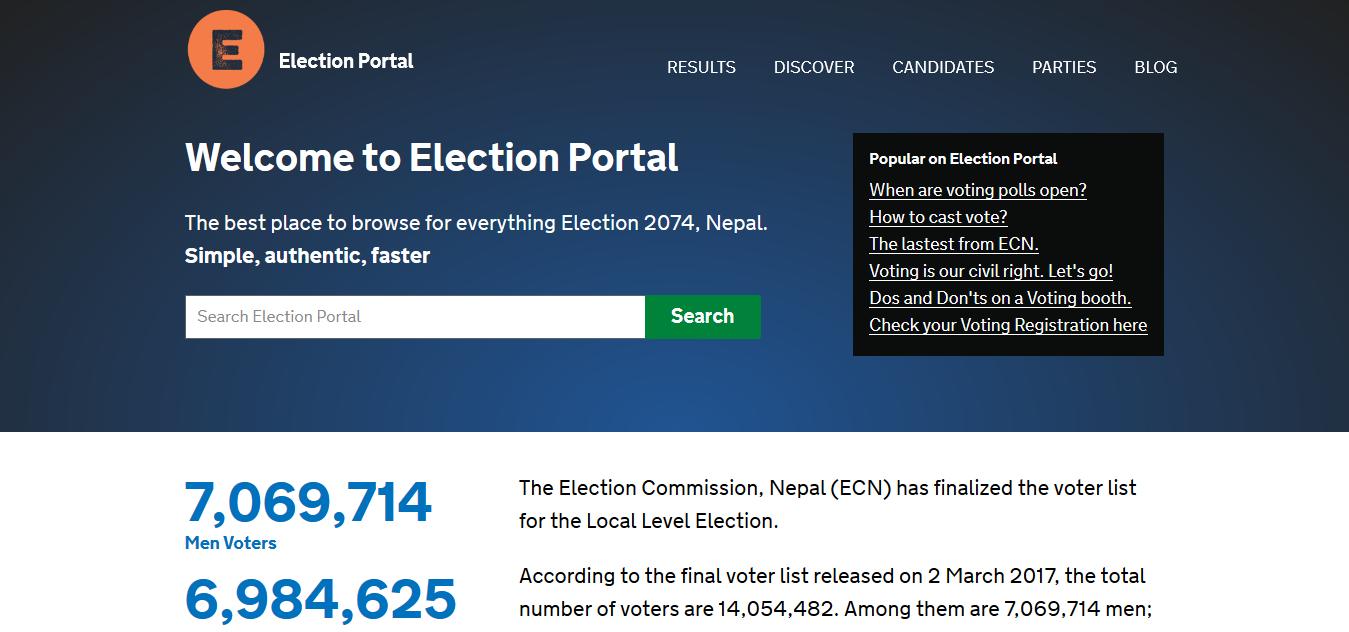
\includegraphics[scale=0.3]{home.png}\\
\end{center}
Besides header and footer, Homepage of Election Portal has a search form which allows visitors to search election datasets without pain. The homepage has a map, so any users can filter the datasets via district.

\subsection{List of Political Party}
All the political parties registered will be listed here along with their party image. Given figure shows same image because we don't have update the database with real datas.\\
\begin{center}
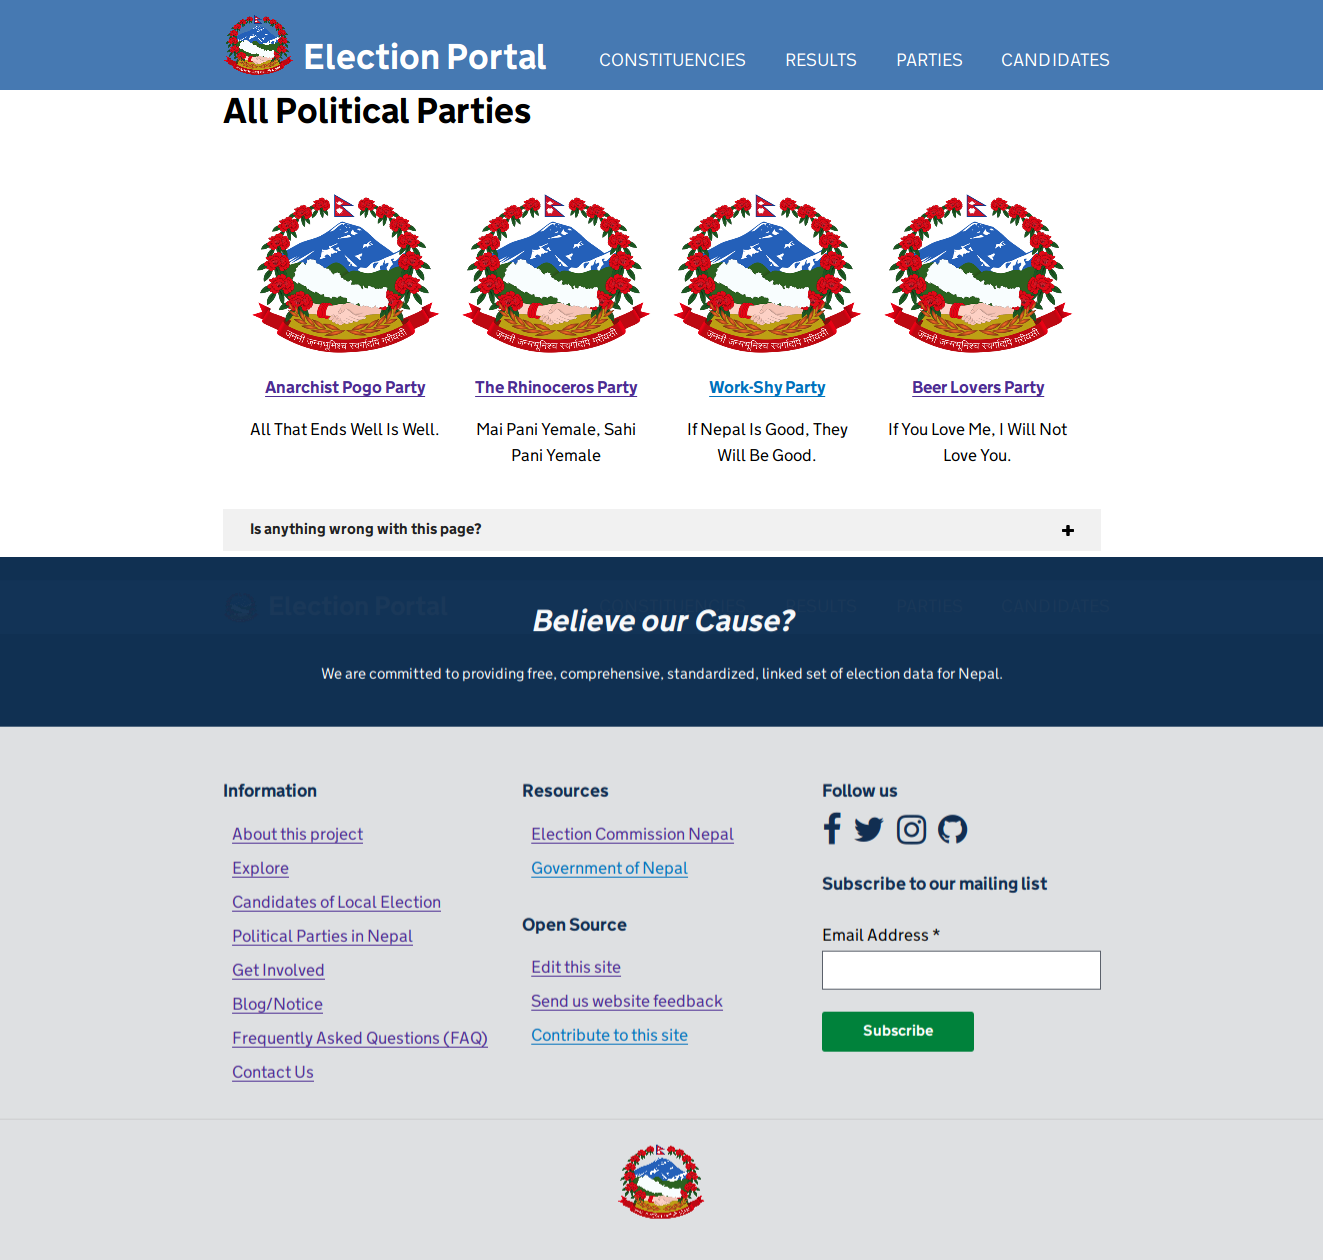
\includegraphics[scale=0.3]{List_of_Political_Party.png}\\
\end{center}

\subsection{Details of Political Party}
\begin{center}
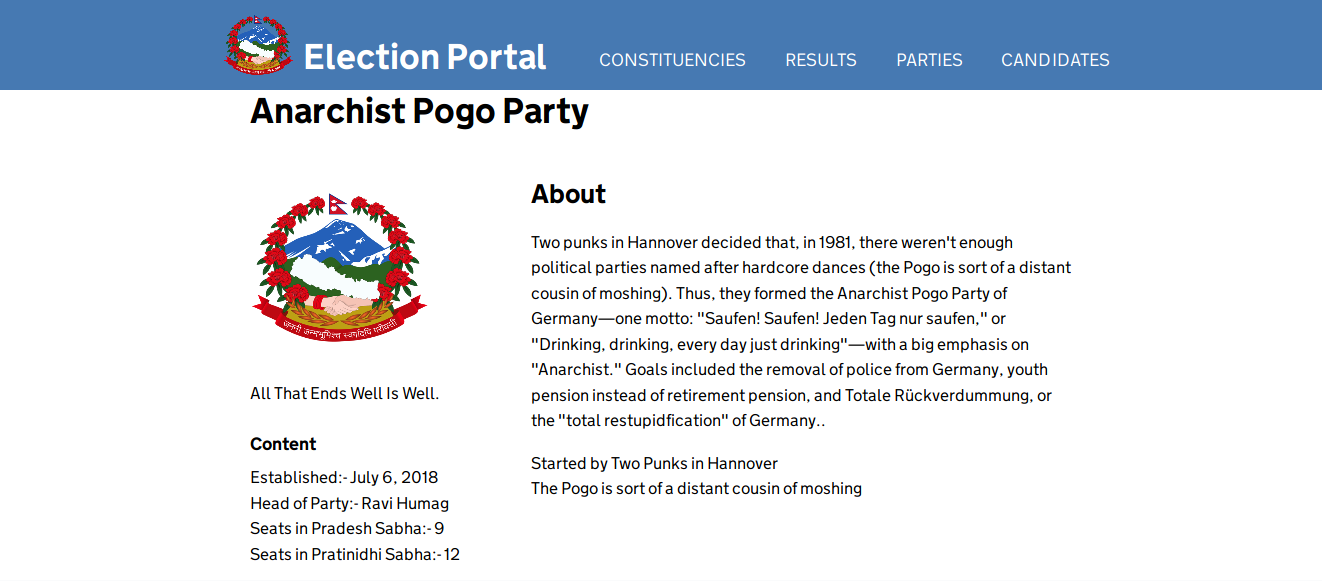
\includegraphics[scale=0.35]{Details_of_Political_Party.png}
\end{center}

\subsection{Details of Nominee}
\begin{center}
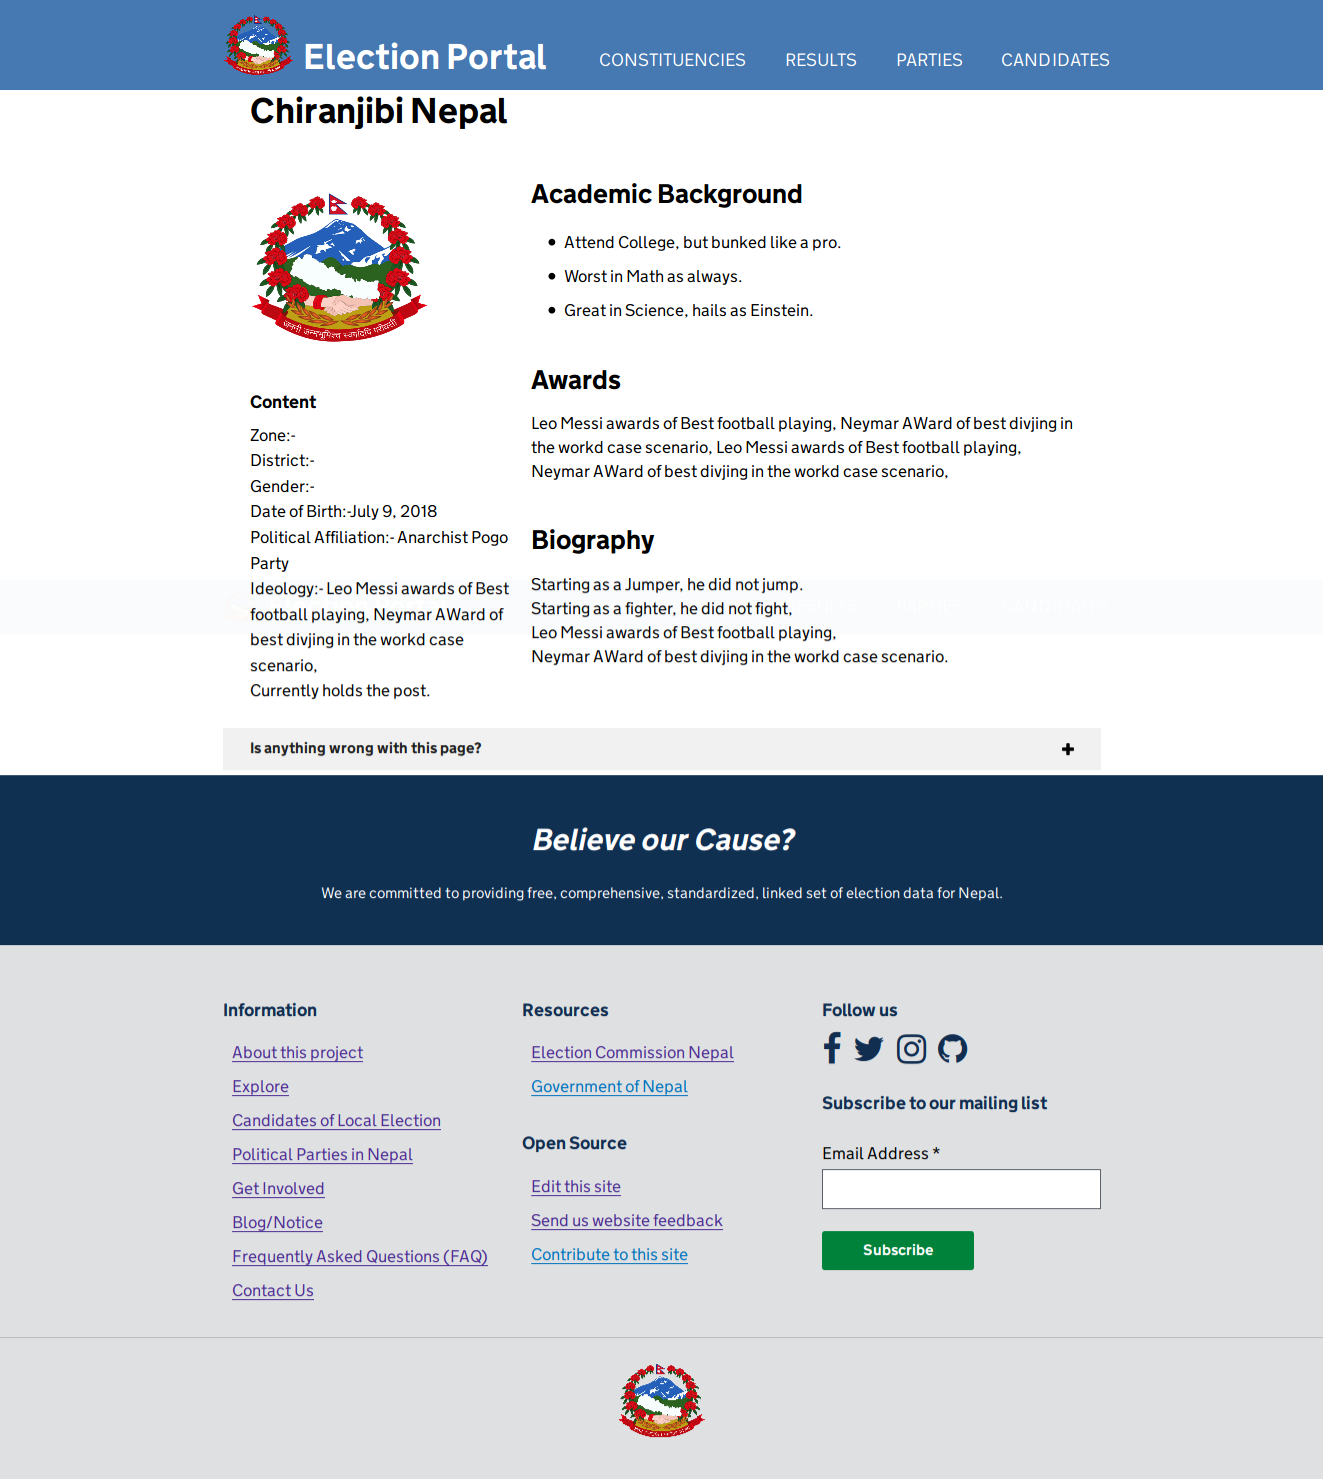
\includegraphics[scale=0.35]{Details_of_a_nominee.png}
\end{center}


\subsection{Details of Constituency}
\begin{center}
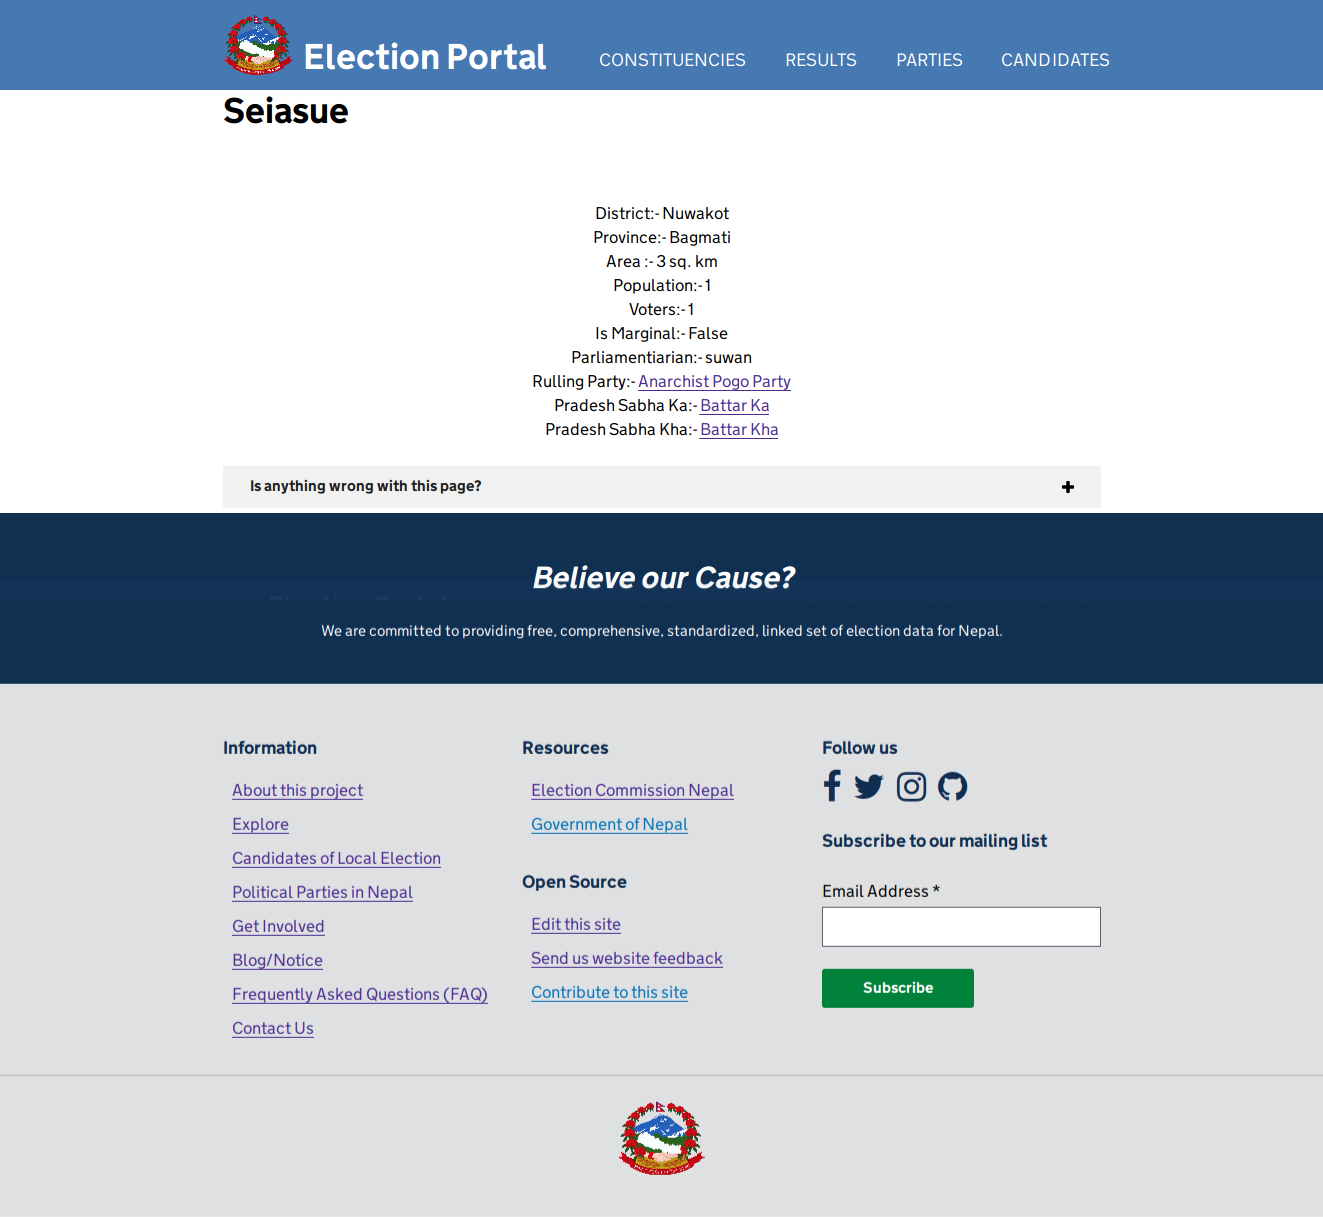
\includegraphics[scale=0.35]{Details_of_Constituency.png}
\end{center}

\begin{appendices}
\section{Installation}
\subsection{Installing Python}

Election Portal is a django app. Django is written in Python, so it requires us to install Python to run the app. For the further note, Django requires Python 2.3 or higher. \\ \\
\textbf{Note:} If you’re on Linux or Mac OS X, you probably already have Python installed.

\subsection{Creating an isolated Python environment}
A virtual environment (also called a virtualenv) is like a private box where developers can stuff useful computer code into for a project they're working on. It is recommended to use virtualenv to create isolated Python environments, because it enables the use of different package versions for different projects, which is far more practical than installing Python packages system wide.
\begin{enumerate}
\item After installing Python Interpreter, we need to install \verb|pip| which is a package management system used to install and manage software packages written in Python.     

\item Let us install \verb|virtualenv| which is required to set up different environments and create an environment named \verb|myenvironment|
\begin{center}
\verb|pip install virtualenv|
\verb|virtualenv myenvironment|
\end{center}
\end{enumerate}

\subsection{Setting up Election Portal on Virtual Environment}
Once we've installed and created the virtual environment, the environments needs to be activated and the dependencies for the application has to be installed. In the next few steps, we'll learn how to install Election Portal on your system.
\begin{enumerate}
\item Now we've created an virtual environment, it has to be activated which is done by
\begin{center}
\verb|source myenvironment/bin/activate|
\end{center}

\item Once the virtual environment is active, we can install the dependencies of the Election Portal app which are located at \verb|requirements.txt|. Election Portal app needs following packages to fully function. 
\begin{lstlisting}
chardet==3.0.4
Django==2.0.7
doc8==0.8.0
docutils==0.14
pbr==4.0.4
pkg-resources==0.0.0
pytz==2018.5
restructuredtext-lint==1.1.3
six==1.11.0
stevedore==1.28.0
django-gfklookupwidget
\end{lstlisting}
All the dependencies can be installed by
\begin{center}
\verb|pip install -r requirements.txt|
\end{center} 
The above steps may require an active Internet Connection. 

\item Change Directory to the Base Directory of Election Portal application \textit{i.e.}, the folder which consists of \verb|manage.py|.

\item Then, run the following commands in your terminal.
\begin{center}
   \verb|python manage.py collectstatic| \\
   \verb|python manage.py makemigrations|\\
   \verb|python manage.py migrate|\\
\end{center}

\item We are all set now. Let's verify if Election Portal works.
\begin{center}
   \verb|python manage.py runserver| \\
\end{center}
\end{enumerate}  
    
\newpage
\end{appendices}




\begin{thebibliography}{9}
 
\bibitem{UCD}
Wikipedia - Use Case Diagram
\\\texttt{https://en.wikipedia.org/wiki/Use-case-diagram}

\bibitem{CD}
Wikipedia - Class Diagram
\\\texttt{https://en.wikipedia.org/wiki/Class-diagram}

\bibitem{Project Report}
Fedrous - Web Design Report
\\\texttt{https://slideshare.net/ferdous/web-design-project-report}
 
\bibitem{Django Website} 
Django Documentation:,
\\\texttt{https://docs.djangoproject.com/en/2.0/}
\end{thebibliography}

\end{document}
         